\documentclass[14pt,a4paper]{article}

\usepackage[UTF8]{ctex}
\usepackage[margin=1.8cm]{geometry}
\usepackage{amsmath,amssymb,booktabs,graphicx,hyperref,enumitem,fancyhdr,listings,float,minted,bookmark}
\usepackage{titlesec}
\usepackage[most]{tcolorbox}
\titleformat{\section}{\centering\LARGE\bfseries}{\thesection}{1em}{}
\pagestyle{fancy}
\fancyhf{}
\fancyhead[L]{\textbf{2025 - 1024 PDCC}}
\fancyhead[R]{\bf Page \thepage}
\renewcommand{\headrulewidth}{0.4pt}
\setCJKmainfont{FandolSong}

\setlength{\parindent}{0pt}
\setlength{\parskip}{0.5em}
\linespread{1.2}
\setlist[itemize]{itemsep=0pt, topsep=2pt}
\setlist[enumerate]{itemsep=0pt, topsep=2pt}


\lstset{
  basicstyle=\ttfamily\small,
  breaklines=true,
  frame=single,
  numbers=left,
  numberstyle=\tiny,
  backgroundcolor=\color[gray]{0.96},
  xleftmargin=1.5em,
}
\newtcolorbox{hintbox}{
  enhanced,
  colback=blue!5!white, 
  colframe=blue!50!black,
  fonttitle=\bfseries,      % 标题加粗
  coltitle=white,           % 标题颜色
  title=Hint,               % 框标题
  sharp corners,
  boxrule=0.5pt,
  left=6pt, right=6pt, top=6pt, bottom=6pt,
  before skip=10pt, after skip=10pt,
  breakable,                % 允许跨页
}

\begin{document}

\begin{center}
  {\Huge \bfseries 1024 Coding Challenge}\\[1em]
  {\Huge \bfseries Algorithmic Track}\\[1em]
  { \Large 2025 Programmer's Day }\\[2em]
  {\Large Full Solution}\\[1em]
\end{center}


\begin{table}[htbp]
  \centering
  \setlength{\tabcolsep}{8pt}  % 列间距
  \renewcommand{\arraystretch}{1.3} % 行距
  \begin{tabular}{|c|c|c|c|c|c|}
    \hline
     题号 & 题目名称 & 通过人数 & 总人数 & 过题率  \\ \hline % 第1行
     A& 台风 & 22 & 22 & 100\% \\ \hline % 第2行
     B& Run-length Encoding & 19 & 22 & 86.3\%  \\ \hline % 第3行
     C& 神秘的三角形 & 14 & 22 & 63.6\%  \\     \hline % 第4行
     D& 图书整理计划 & 14 & 22 & 63.6\% \\ \hline % 第5行
     E& Fetch-Decode-Execute & 5 & 22 & 22.7\%  \\ \hline % 第6行
     F& 不神秘构造题 & 8 & 22 & 36.4\% \\ \hline % 第7行
     G& 星辉廊道 & 4 & 22 & 18.2\%  \\ \hline % 第8行
     H& File Restoration & 4 & 22 & 18.2\%  \\ \hline % 第9行
     I& 扫雷 & 3 & 22 & 13.6\%  \\ \hline % 第10行
     J& $1024_{1024}$ Puzzle & 3 & 22 & 13.6\%  \\ \hline % 第11行
     K& 抽卡打怪 & 2 & 22 & 9.1\%  \\ \hline % 第12行
     L& 「星光渐明之时」 & 2 & 22 & 9.1\%  \\ \hline % 第13行
  \end{tabular}
\end{table}

{ \Large \bfseries Staff 如是说:}
\begin{itemize}
    \item Allen: L 题通过率有点小高哈,这道题本来有 puzzle 元素的结果后面被砍掉了(悲。不过看大家做题还是很爽的!orz orz jhd \& wowo AK!
\end{itemize}
\clearpage

\section{台风}
签到题,输出 \texttt{Reject!} 即可。

\section{神秘的三角形}
签到题,建议用 python 避免精度出问题。

\section{图书馆整理计划}
签到题,输出 $\left(\sum_{i=1}^{n} a_i\right)/B\times X + \left(\sum_{i=1}^{n} a_i\right) \times Y \bmod B $ 即可。

\section{Fetch-Decode-Execute}
出题人的语文水平过于低下导致这道小模拟变成阅读理解,没什么特别需要解释的,放个std。python可能会超时
\begin{minted}{cpp}
#include <bits/stdc++.h>
using namespace std;

struct Instruction {
    string op;
    int arg;
};

int main() {
    ios_base::sync_with_stdio(false);
    cin.tie(NULL);

    int n;
    cin >> n;

    vector<Instruction> prog;
    prog.reserve(n);

    for (int i = 0; i < n; ++i) {
        string op_str;
        cin >> op_str;

        int arg_val = 0;
        if (op_str != "NOP" && op_str != "HALT") {
            cin >> arg_val;
        }
        prog.push_back({op_str, arg_val});
    }

    int A = 0;
    vector<int> D(256, 0);
    int PC = 0;
    long long cycles = 0;
    const int MAX_CYCLES = 10000000;
    string reason;

    while (true) {
        if (cycles >= MAX_CYCLES) {
            reason = "TIMEOUT";
            break;
        }

        if (PC < 0 || PC >= n) {
            reason = "CRASH";
            break;
        }

        string op = prog[PC].op;
        int arg = prog[PC].arg;
        cycles++;
        int next_pc = PC + 1;

        if (op == "LOAD") A = D[arg];
        else if (op == "STORE") D[arg] = A;
        else if (op == "ADD") A += D[arg];
        else if (op == "SUB") A -= D[arg];
        else if (op == "MUL") A *= D[arg];
        else if (op == "MOV") A = arg;
        else if (op == "JMP") next_pc = arg;
        else if (op == "JZ") {
            if (A == 0) next_pc = arg;
        } else if (op == "JNZ") {
            if (A != 0) next_pc = arg;
        } else if (op == "NOP") {
        } else if (op == "HALT") {
            reason = "HALT";
            break;
        }

        PC = next_pc;
    }

    cout << reason << endl;
    cout << A << endl;
    cout << cycles << endl;

    return 0;
}
\end{minted}


\section{星辉廊道}
显然,本题可以被简单的化简为\textbf{最大化路径上所有边权的按位与}。

\begin{hintbox}
考虑按位与运算的性质:若结果的某一位为 $1$,则路径上所有边该位都必须为 $1$。
\end{hintbox}

我们可以采用按位枚举的套路确定答案。

具体而言,我们从高位往低位逐步构造答案 $\text{ans}$:

\begin{enumerate}
  \item 初始 $\text{ans}=0$。
  \item 从第 $29$ 位到第 $0$ 位,对于每一位 $b$):
  \begin{itemize}
  \item 令 $\text{test} \leftarrow \text{ans} \lor (1 \ll b)$,假设当前位为 $1$。
  \item 仅保留所有满足 $(w \land \text{test}) = \text{test}$ 的边(即选择所有在第 $b$ 位上是 $1$ 的边)。
  \item 在这个新图中暴力 BFS 检查 $1$ 是否能到达 $N$。
  \item 若能到达,则说明该位可以保留,更新答案;否则该位不能保留,保持答案不变。
  \end{itemize}
\end{enumerate}

\begin{minted}{cpp}
signed main(){
    cin.tie(nullptr)->sync_with_stdio(0);
    cin>>n>>m;
    for(int i=1;i<=m;i++){
        int u,v,w;cin>>u>>v>>w;
        add(u,v,w),add(v,u,w);
    }
    auto chk=[&](int flag){
        vector<int> vis(n+1,0);
        queue<int> q; vis[1]=1; q.push(1);
        while(!q.empty()){
            int u=q.front();q.pop();
            for(int i=head[u];i;i=edge[i].next){
                int v=edge[i].to, w=edge[i].w;
                if(!vis[v] && ((w&flag)==flag)){
                    vis[v]=1;
                    q.push(v);
                }
            }
        }
        return vis[n];
    };
    for(int s=29;s>=0;s--){
        int tmp=cnt|(1<<s);
        if(chk(tmp)) cnt=tmp;
    }
    cout<<cnt;
    return 0;
}
\end{minted}

\section{File Restoration}
又是一道小清新 DP 好题!Allen 太喜欢 DP 了(什

观察题面,一个很好的思路是将每一个文件夹抽象为一个节点,则整个文件夹目录可以被视作一棵树。

考虑如何设计状态以及如何进行树上转移。

由于两种操作一种是单点翻转一种是子树翻转,我们从相对来说较难的子树翻转入手。

\paragraph{状态}
子树翻转每次都会将一个父节点的所有子节点以及其本身直接翻转,因此 DP 状态中肯定需要一个东西去记录和转移继承下来的翻转信息。

设 $p\in\{0,1\}$ 为到达当前节点时,因父节点的 “子树翻转” 累积到它身上的翻转奇偶。

$dp_{u,p}$ 就可以被设计为:

\textbf{在节点 $u$,在已承受奇偶为 $p$ 的情况下,让 $u$ 的整棵子树全为 $1$ 的最小操作数。}

\paragraph{转移}
有了状态,转移就是 trivial 的了。

我们仅需在 $u$ 处决定是否做一次“以 $u$ 为根的子树翻转”。

记该决策 $y\in\{0,1\}$,做了之后传下去的懒标记变为 $p' = p\oplus y$。

$v$ 的当前值变成 $a_v\oplus p'$。若为 $0$,需要再做一次 “单点翻转 $v$”。

子树代价显然是 $\sum_{\forall \text{son}} dp_{\text{son},p'}$。

\begin{minted}{cpp}
int arr[maxn];
vector<int> e[maxn];
int dp[maxn][2];

void dfs(int u, int fa){
    for(int v:e[u]){
        if(v!=fa) dfs(v,u);
    }
    for(int p=0;p<=1;p++){
        int best=1e9+7;
        for(int y=0;y<=1;y++){
            int flag=arr[u]^p^y^1;
            int cost=y+flag;
            for (int v:e[u]){
                if(v!=fa) cost+=dp[v][p^y];
            }
            best=min(best,cost);
        }
        dp[u][p]=best;
    }
}

signed main(){
    cin.tie(nullptr)->sync_with_stdio(0);
    cin>>n;
    for(int i=1;i<=n;i++) cin>>arr[i];
    for(int i=1;i<=n-1;i++){
        int u,v;cin>>u>>v;
        e[u].pb(v);e[v].pb(u);
    }
    dfs(1,0);
    cout<<dp[1][0]<<endl;
    return 0;
}
\end{minted}

\section{抽卡打怪}
来一发验题人题解。

\section{「星光渐明之时」}
\textbf{本篇题解包含医疗建议。(x}

这应该是本场比赛里最好的一道思维 + DS 题!

部分分能给我们很大的启发。

\subsection{Subtask 1}
给了 $8$ 分的暴力分,但是可能普通暴力过不去,因为带修改情况下 $a_i$ 有一定概率超过给定值域 $V = 10^9$,也有可能会爆 long long。

\subsection{Subtask 2}

\begin{hintbox}
不妨先思考这道题不带修改怎么做。
\end{hintbox}

把题面简化为:

给定序列 $a_1, \dots, a_n$,对于区间 $[l,r]$,询问最少需要多少次操作,才能使得 $a_l, \dots, a_r$ 不降。

为了方便计数,我们定义第 $i$ 个数乘 $2$ 的次数为 $e_i \in \mathbb{Z}_{\ge 0}$。

询问的目标是最小化:

\begin{equation}
    \sum_{i=l+1}^{r} e_i \quad \text{s.t.} \quad a_i\times 2^{e_i} \le a_{i+1}\times 2^{e_{i+1}} \quad (\forall i \in [l, r-1]).
    \label{eq:goal1}
\end{equation}


把相邻约束用指数差线性化。定义
\begin{equation}
    c_i = \left \lceil \log_2 \frac{a_{i}}{a_{i-1}} \right \rceil \in \mathbb{Z} \quad (i \in [2,n])
\end{equation}
则
\begin{equation}
    a_i\times 2^{e_i} \le a_{i+1}\times 2^{e_{i+1}} \iff e_{i+1} - e_i \ge c_i.
\end{equation}

于是~\eqref{eq:goal1} 可被重写为
\begin{equation}
    \sum_{i=l+1}^{r} e_i \quad \text{s.t.} \quad e_{i+1} - e_i \ge c_i, e_i \ge 0.
    \label{eq:goal2}
\end{equation}

令前缀和
\begin{equation}
    s_k = \sum_{i=1}^{k} c_i.
\end{equation}

容易得到我们最后的结论:

\begin{equation}
    \text{Ans}(l,r) = \sum_{k=l+1}^{r} (s_k - \min_{t \in [l+1, k]} s_t).
    \label{eq:ans}
\end{equation}

\paragraph{证明}

令 $t^* = \arg \min_{t\in[l+1,k]} s_t$。

则由~\eqref{eq:goal2} 我们有
\begin{equation}
    e_k - e_{t^*} \ge \sum_{i=t^*}^{k-1} c_i = s_k - s_{t^*}
\end{equation}

由于 $e_{t^*} \ge 0$,那么

\begin{equation}
    e_k \ge s_k - \min_{t\in[l+1,k]} s_t
\end{equation}

取等并累加时即是最小值,证毕。

问题来了,怎么实现这个算法呢?

观察 $s_i$ 图像:

\begin{figure}[H]
    \centering
    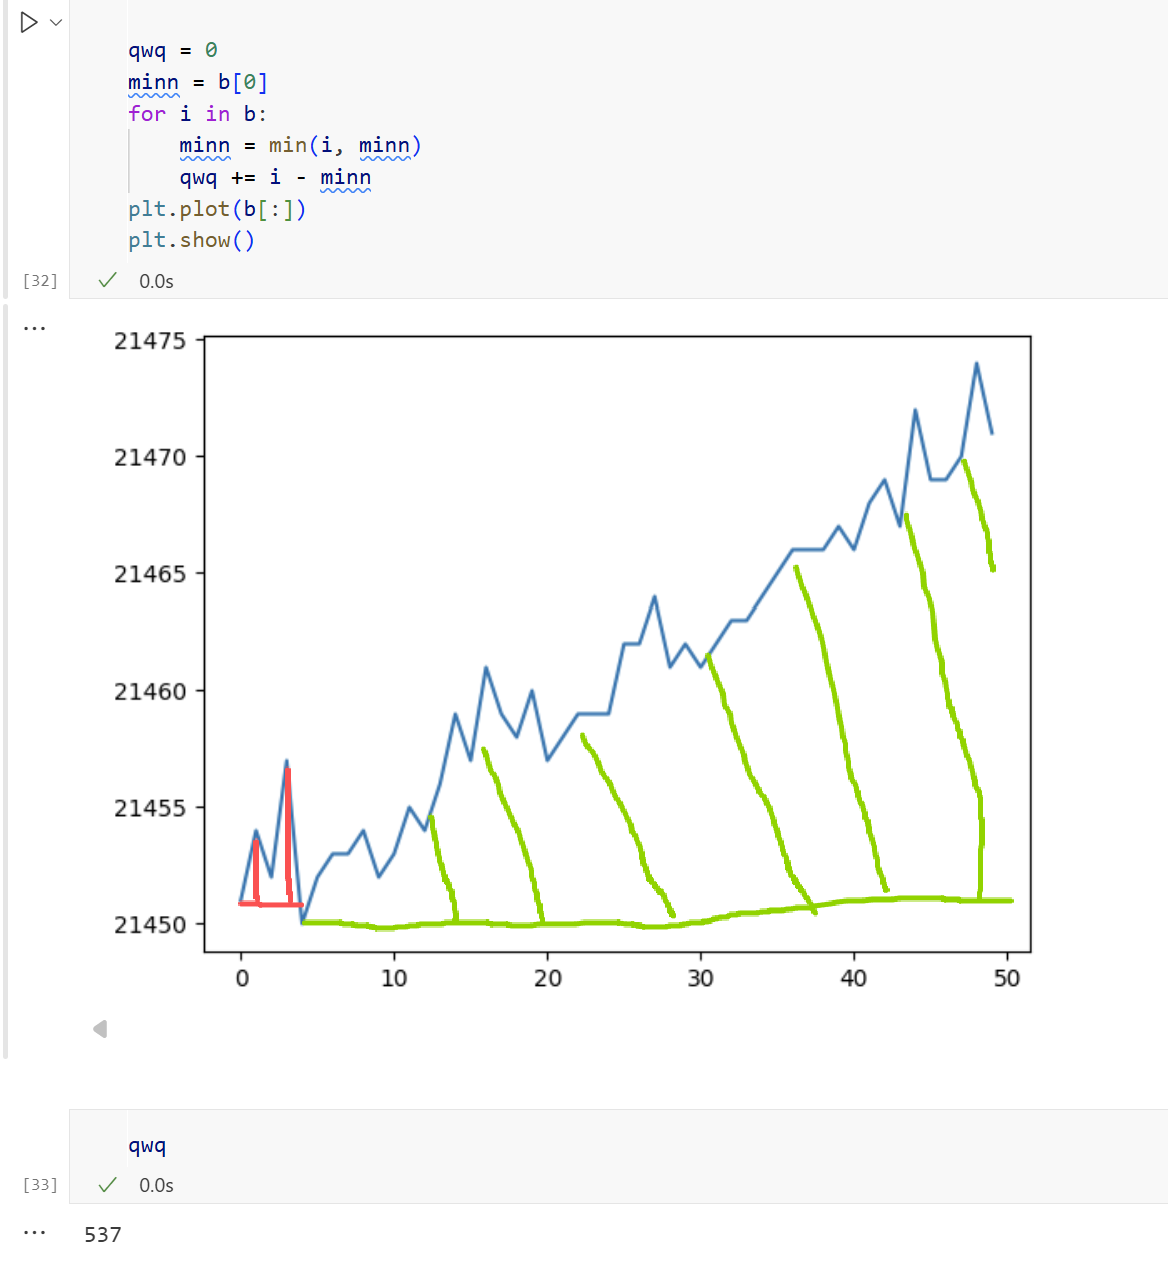
\includegraphics[width=0.5\textwidth]{image.png}
\end{figure}

我们不难发现我们最后的答案就是图像中标出来的东西,由多个 $\min$ 分界点对应区间的贡献合并而成。

我们可以用一个单调栈来维护这些分界点,加上前缀和的预处理,每次询问时暴力遍历所有分界点,统计答案即可。

时间复杂度显然正确,因为在不带修改的情况下,分界点的数量不会超过 $O(\log_2 V)$ ($\min s_t$ 最多被“刷新” $O(\log_2 V)$ 次),在随机数据下常数很小,跑的很快。

这一部分给了 24 分的部分分。

\subsection{Subtask 3}
然而,在带修改以及强制在线情况下,我们不能使用单调栈,因此需要一个数据结构来维护信息。

考虑修改操作对序列 $s_i$ 的影响。

简单手摸几组 sample 就可以知道,对 $a_i$ 进行一次修改仅会减少 $s_i$,值恒定为 $1$。

对于\textbf{前缀和}的维护,我们可以简单的使用常数小的树状数组。
而对于\textbf{分界点}的维护,我们可以使用线段树。

具体而言,我们只需要实现一个函数 $\text{queryFirst}(x) $,返回第一个满足 $s_i \le x$ 的位置 $i$ 即可,该位置即是我们所需的分界点。

带修改后,单次查询期望时间复杂度退化为 $O(\sqrt{n} \times \log_2 n)$($n,q$ 同阶,证明略),常数超级小就是了,跑的飞快。

当然,\eqref{eq:ans} 可以直接套单侧递归线段树做,单次复杂度直接进化为 $O(\log_2^2 n)$,但是实测常数很大,跑的比 sqrt 慢就是了(验题人以及 wowo 都是此类写法)。

后面的事情就是 trivial 的了。

\begin{minted}{cpp}
int arr[maxn], brr[maxn];

struct BIT{
    int n;vector<int> brr;
    BIT(int range){n=range;brr.resize(n+1,0);}
    int lowbit(int x){return x&(-x);}
    inline void add(int x, int k){while(x<=n){brr[x]+=k;x+=lowbit(x);}}
    inline int query(int x){int ans=0;while(x!=0){ans+=brr[x];x-=lowbit(x);}return ans;}
    inline int queryRange(int l, int r){return query(r)-query(l-1);}
};

struct info{
    int ls,rs;
    int tagMin;
}tree[maxn<<3];

void buildTree(int &p, int pl, int pr){
    p=++cnt;
    if(pl==pr){
        tree[p]=(info){0,0,brr[pl]};
        return;
    }
    int mid=(pl+pr)>>1;
    buildTree(tree[p].ls,pl,mid);
    buildTree(tree[p].rs,mid+1,pr);
    tree[p].tagMin=min(tree[tree[p].ls].tagMin,tree[tree[p].rs].tagMin); //pushup
}

void addPoint(int p, int x, int pl, int pr){
    if(pl==pr){
        tree[p].tagMin--;
        return;
    }
    int mid=(pl+pr)>>1;
    if(x<=mid) addPoint(tree[p].ls,x,pl,mid);
    else addPoint(tree[p].rs,x,mid+1,pr);
    tree[p].tagMin=min(tree[tree[p].ls].tagMin,tree[tree[p].rs].tagMin); //pushup
}

int queryFirst(int p, int pl, int pr, int l, int r, int x){
    if(r<pl || pr<l || x<=tree[p].tagMin) return n+1;
    if(pl==pr) return pl;
    int mid=(pl+pr)>>1;
    int res=n+1;
    if(l<=mid){
        res=queryFirst(tree[p].ls,pl,mid,l,r,x);
    }
    if(res==(n+1) && r>mid){
        res=queryFirst(tree[p].rs,mid+1,pr,l,r,x);
    }
    return res;
}

signed main(){
    cin.tie(nullptr)->sync_with_stdio(0);
    cin>>n>>m;
    for(int i=1;i<=n;i++){
        cin>>arr[i];
    }
    for(int i=2;i<=n;i++){
        int x=arr[i-1],y=arr[i];
        while(x<=y/2) x<<=1,brr[i]--;
        while(x>y) y<<=1,brr[i]++;
    }
    BIT bit(n);
    for(int i=2;i<=n;i++){
        brr[i]+=brr[i-1];
        bit.add(i,brr[i]);
    }
    int root=0;
    buildTree(root,1,n);
    auto query=[&](int l, int r){
        int pos=l-1,ans=0;
        while(pos<r){
            int to=queryFirst(root,1,n,pos+1,n,brr[pos])-1;
            if(to>r){
                ans+=bit.queryRange(pos+1,r)-(r-pos)*bit.queryRange(pos,pos);
                break;
            }
            ans+=bit.queryRange(pos+1,to)-(to-pos)*bit.queryRange(pos,pos);
            pos=to+1;
        }
        return ans;
    };
    while(m--){
        int op;cin>>op;
        if(op==1){
            int x;cin>>x;
            addPoint(root,x,1,n);brr[x]--;
            bit.add(x,-1);
        }else{
            int l,r;cin>>l>>r;l++;
            cout<<query(l,r)<<endl;
        }
    }
    return 0;
}
\end{minted}
\end{document}